\documentclass{ctexart}
\textheight 23.5cm \textwidth 15.8cm
\topmargin -1.5cm \oddsidemargin 0.3cm \evensidemargin -0.3cm

\usepackage{verbatim}
\usepackage{fancyhdr}
\usepackage{float}
\usepackage{graphicx}
\usepackage{amssymb}
\usepackage{amsmath}


\pagestyle{fancy}
\CTEXsetup[format = {\Large\bfseries\it}]{section}


\begin{document}

\section*{内容简介}
	\begin{itemize}
		\item 画出五阶 Adams-Bashforth 公式和五阶 Adams-Moulton 公式的绝对稳定性区域
		\item 使用Mathematica绘制,使用ImplicitPlot函数
	\end{itemize}

	
\section*{输出结果}
	\begin{figure}[H]
		\centering
		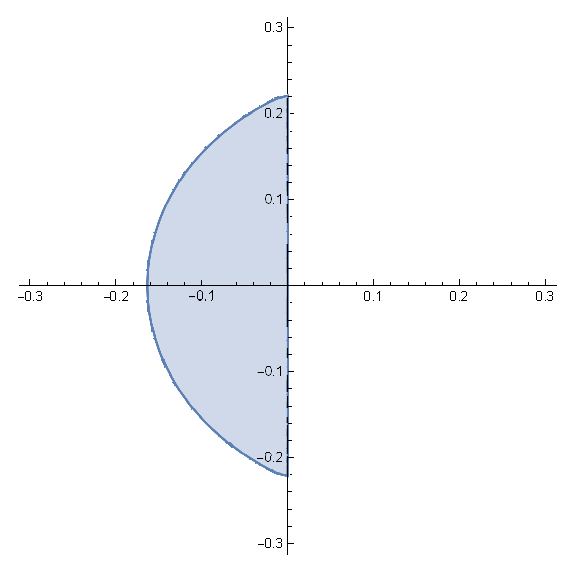
\includegraphics[width = 10cm, height = 8cm]{Adams-Bashforth-5.eps}
		\caption{五阶 Adams-Bashforth 公式的绝对稳定性区域} \label{figure-1.label}
	\end{figure}
	
	\begin{figure}[H]
		\centering
		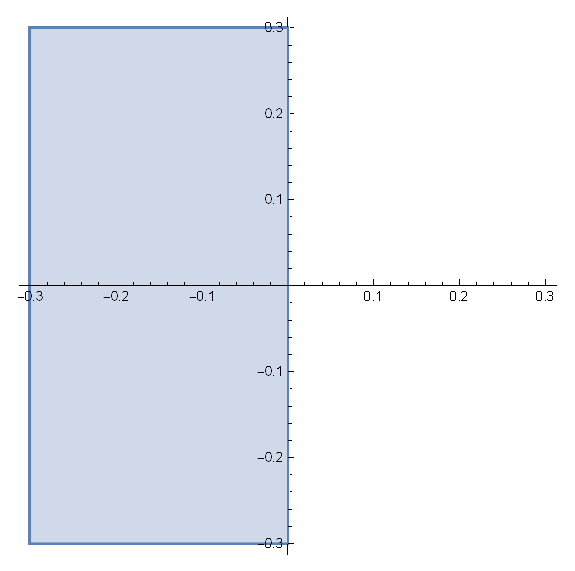
\includegraphics[width = 10cm, height = 8cm]{Adams-Moulton-5.eps}
		\caption{五阶 Adams-Moulton 公式的绝对稳定性区域} \label{figure-2.label}
	\end{figure}


\section*{分析}
	一般的线性多步法有下列性质:
	\begin{equation}
		a_k y_n + a_{k-1} y_{n-1} + \cdots + a_0 y_{n-k} = h \lambda (b_k f_n + b_{k-1} f_{n-1} + \cdots + a_0 f_{n-k})
	\end{equation}
	应用于试验方程
	\begin{equation}
	\begin{cases}
		y' = \lambda y\\
		y(0) = s
	\end{cases}
	\end{equation}
	得到
	\begin{equation}
		a_k y_n + a_{k-1} y_{n-1} + \cdots + a_0 y_{n-k} = h \lambda (b_k y_n + b_{k-1} y_{n-1} + \cdots + a_0 y_{n-k})
	\end{equation}
	对应于求解齐次线性差分方程
	\begin{equation}
		(a_k - h \lambda b_k) y_n + (a_{k-1} - h \lambda b_{k-1}) y_{n-1} + \cdots + (a_0 - h \lambda b_0) y_{n-k} = 0
	\end{equation}
	其解为形如 $y_n = r^n$ 的一些基本解的线性组合,其中 $r$ 是多项式 $\phi$ 的一个根。$\phi$ 具有性质:
	\begin{align*}
		\phi & = p - \lambda h q \\
		p(z) & = a_k z^k + a_{k-1} z^{k-1} + \cdots + a_1 z + a_0 \\
		q(z) & = b_k z^k + b_{k-1} z^{k-1} + \cdots + b_1 z + b_0
	\end{align*}
	
	只有当所有根满足 $|r| < 1$,数值解才能保证具有衰减性质($y_n \rightarrow 0$,当 $n \rightarrow \infty$)。使得多项式 $\phi$ 的所有根均落在圆盘 $|z| < 1$ 中的 $\omega = \lambda h$ 的取值区域即 {\bf 绝对稳定性区域}。
	
\section*{参考资料}
	\noindent [1] David R. Kincaid \& E. Ward Cheney. {\it Numerical Analysis: Mathematics of Scientific of Computing Third Edition}, Brooks/Cole, 2002.
	
\end{document}